\documentclass[10pt,a4paper]{article}
\usepackage[UTF8,fontset = windows]{ctex}
\setCJKmainfont[BoldFont=黑体,ItalicFont=楷体]{华文中宋}
\usepackage{amssymb,amsmath,amsfonts,amsthm,mathrsfs,dsfont,graphicx}
\usepackage{ifthen,indentfirst,enumerate,color,titletoc}
\usepackage{tikz}
\usepackage{makecell}
\usepackage{longtable}

\usetikzlibrary{arrows,calc,intersections,patterns}
\usepackage[bf,small,indentafter,pagestyles]{titlesec}
\usepackage[top=1in, bottom=1in,left=0.8in,right=0.8in]{geometry}
\renewcommand{\baselinestretch}{1.65}
\newtheorem{defi}{定义~}
\newtheorem{eg}{例~}
\newtheorem{ex}{~}
\newtheorem{rem}{注~}
\newtheorem{thm}{定理~}
\newtheorem{coro}{推论~}
\newtheorem{axiom}{公理~}
\newtheorem{prop}{性质~}
\newcommand{\blank}[1]{\underline{\hbox to #1pt{}}}
\newcommand{\bracket}[1]{(\hbox to #1pt{})}
\newcommand{\onech}[4]{\par\begin{tabular}{p{.9\textwidth}}
A.~#1\\
B.~#2\\
C.~#3\\
D.~#4
\end{tabular}}
\newcommand{\twoch}[4]{\par\begin{tabular}{p{.46\textwidth}p{.46\textwidth}}
A.~#1& B.~#2\\
C.~#3& D.~#4
\end{tabular}}
\newcommand{\vartwoch}[4]{\par\begin{tabular}{p{.46\textwidth}p{.46\textwidth}}
(1)~#1& (2)~#2\\
(3)~#3& (4)~#4
\end{tabular}}
\newcommand{\fourch}[4]{\par\begin{tabular}{p{.23\textwidth}p{.23\textwidth}p{.23\textwidth}p{.23\textwidth}}
A.~#1 &B.~#2& C.~#3& D.~#4
\end{tabular}}
\newcommand{\varfourch}[4]{\par\begin{tabular}{p{.23\textwidth}p{.23\textwidth}p{.23\textwidth}p{.23\textwidth}}
(1)~#1 &(2)~#2& (3)~#3& (4)~#4
\end{tabular}}
\begin{document}
\begin{enumerate}[1.]

%1_21
\item 设$A=\{x|x^2-6x+5\le 0\}$, $B=\{2,3,4,5,6,7\}$, 则$A\cap B=$\blank{50}.
\item 已知函数$f(x)=\lg (x+1)$的反函数为$y=f^{-1}(x)$, 则$f^{-1}(2)=$\blank{50}.
\item 设$\mathrm{i}$是虚数单位, 若$z+2\overline z=3+4\mathrm{i}$, 则$2z+\overline z=$\blank{50}.
\item 若$f(x)$是奇函数, 且当$x\ge 0$时, $f(x)=x^2+x$, 则当$x<0$时, $f(x)=$\blank{50}.
\item 设$A,B,C$是三角形的三个内角, 若$(\sin A+\sin B)^2-{{\sin }^2}C=3\sin A\sin B$, 则$C=$\blank{50}.
\item 若一组数据$2,3,a,b,7,9$的中位数为$8$, 则$a+b$的最小值为\blank{50}.
\item $(2+x)^6$的二项展开式中, 系数最大的项的系数为\blank{50}.
\item 设$A,B$是一条斜率为$4$的直线与抛物线$y^2=x$的两个交点, 则线段$AB$的中点的坐标可能是\blank{50}(写出一个可能的点的坐标).
\item 等差数列$\{a_n\}$中, $a_{20}<0$, $a_{21}>0$, 且$a_{20}+a_{21}>0$. 设$S_n$是数列$\{a_n\}$的前$n$项和, 若$S_k>0$, 则正整数$k$的最小值为\blank{50}.
\item 过点$P(2,3)$的直线$l$分别交$x$轴、$y$轴的正半轴于$A$、$B$两点, 则当$|PA|\cdot|PB|$取到最小值时, $l$的方程为\blank{50}.
\item 已知实数$r>0$, 圆$(x-3)^2+(y-4)^2=r^2$上有且仅有两点到直线$3x-4y-2=0$的距离为$1$, 则半径$r$的取值范围为\blank{50}.
\item 已知集合$A=\{x|x=2n-1, \ n\in \mathbf{N}^*\}$, $B=\{x|x=2^k, \ k\in \mathbf{N}^*\}$. 将$A\cup B$的所有元素从小到大依次排列构成一个数列$\{a_n\}$. 记$S_n$为数列$\{a_n\}$的前$n$项和, 则使得$a_n\in A$与${S_{n-1}}>100{a_n}$同时成立的正整数$n$的最小值为\blank{50}.
\item ``函数$y=f(x), \ x\in \mathbf{R}$是增函数''是``函数$y=2-f(x), \ x\in \mathbf{R}$是减函数''的\bracket{20}.
\fourch{充分非必要条件}{必要非充分条件}{充要条件}{既非充分又非必要条件}
\item 银行一年定期的年利率为$r$, 五年定期的年利率为$q$, 银行为吸收长期资金, 鼓励储户存五年定期的存款, 那么$q$的值应略大于\bracket{20}.
\fourch{$\sqrt[5]{(1+r)^5-1}$}{$\dfrac 15((1+r)^5-1)$}{$(1+r)^5-1$}{$r$}\item 设$m$是正实数, 若椭圆$mx^2+(m+1)y^2=1$的两焦点的距离为$3$, 则$m$的值为\bracket{20}.
\fourch{$\dfrac{\sqrt{13}-3}6$}{$\dfrac{\sqrt{21}-3}6$}{$\dfrac 13$}{$\dfrac{\sqrt{33}-3}6$}\item 已知$\overline a,\overline b,\overline e$是平面向量, $\overline e$是单位向量. 若非零向量$\overline a$与$\overline e$的夹角为$\dfrac{\pi}3$, 向量$\overline b$满足$\overline b^2-4\overline e\cdot \overline b+3=0$, 则$|\overline a-\overline b|$的最小值为\bracket{20}.
\fourch{$\sqrt 3-1$}{$\sqrt 3+1$}{$2$}{$2-\sqrt 3$}
\item 在直三棱柱$ABC-A_1B_1C_1$中, $\angle ABC=90^\circ$, $AB=BC=1$.
\begin{center}
    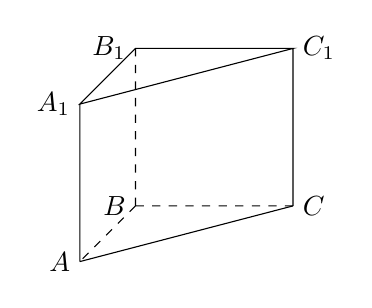
\begin{tikzpicture}
        \draw (0,0) node [left] {$B$} coordinate (B);
        \draw (2,0) node [right] {$C$} coordinate (C);
        \draw (225:1) node [left] {$A$} coordinate (A);
        \draw (A) ++ (0,2) node [left] {$A_1$} coordinate (A1);
        \draw (B) ++ (0,2) node [left] {$B_1$} coordinate (B1);
        \draw (C) ++ (0,2) node [right] {$C_1$} coordinate (C1);
        \draw [dashed] (B) -- (C) (B) -- (A) (B) -- (B1);
        \draw (A) -- (C) (A) -- (A1) (C) -- (C1) (A1) -- (B1) -- (C1) -- cycle;
    \end{tikzpicture}
\end{center}
(1) 若该直三棱柱的表面积为$3+\sqrt 2$, 求直线$A_1C$与平面$ABC$所成的角的大小;\\
(2) 若异面直线$BC$与$AC_1$所成的角的大小为${60}^{^\circ }$, 求该直三棱柱的体积.
\item 已知$a$是常数, 设函数$f(x)=(a-2)x^2+2(a-2)x-4$.\\
(1) 解不等式: $f(x)>-4$;\\
(2) 求实数$a$的取值范围, 使得$f(x)<0$对任意$x\in [1,3]$恒成立;
\item 设函数$f(x)=\cos^2x-2\sin x\cos x+3\sin^2x$.\\
(1) 求使$f(x)$取得最大值的$x$的集合;\\
(2) 设$x_1,x_2\in \mathbf{R}^+$, 且$f(x_1)+f(x_2)=4$. 求证: $x_1+x_2\ge \dfrac{\pi}2$.
\item 若无穷数列$\{a_n\}$满足: 只要$a_p=a_q \ (p,q\in \mathbf{N}^*)$, 必有$a_{p+1}=a_{q+1}$, 则称$\{a_n\}$具有性质$P$.\\
(1) 设数列$\{a_n\}$的通项公式为$a_n=\cos \dfrac{n\pi}{6}$, 判断$\{a_n\}$是否具有性质$P$, 并说明理由;\\
(2) 若$\{a_n\}$具有性质$P$, 且$a_1=1$, $a_2=2$, $a_4=3$, $a_5=2$, $a_6+a_7+a_8=12$, 求$a_3$;\\
(3) 设无穷数列$\{b_n\}$的前三项依次成等比数列, 无穷数列$\{c_n\}$是等差数列, $b_1=c_3=1$, $b_3=c_1=9$. 设$a_n=b_n+c_n\ (n\in \mathbf{N}^*)$. 若$\{a_n\}$具有性质$P$, 求$b_1+b_2+\cdots+b_{30}$.
\item 已知抛物线$C$的方程为$y^2=x$, 圆$M$的方程为$(x-2)^2+y^2=1$.\\
(1) 设$P$是抛物线$C$上的动点, 证明: $P$在圆$M$外;\\
(2) 设斜率为$1$的直线$l$与圆$M$相切, 且与抛物线$C$交于$Q_1,Q_2$两点, 求$|Q_1Q_2|$的值;\\
(3) 设$A_1,A_2,A_3$是抛物线$C$上的三点, 直线$A_1A_2$, 直线$A_1A_3$均与圆$M$相切, 判断直线$A_2A_3$与圆$M$的位置关系, 说明理由.

%2_21
\item 方程$2^x=3$的解为$x=$\blank{50}.
\item 设$z=\dfrac{2-\mathrm{i}}{1+\mathrm{i}}$, 则$|z|=$\blank{50}.
\item 若角$\alpha$的终边过点$P(4,-3)$, 则$\sin(\dfrac{3\pi}2+\alpha)=$\blank{50}.
\item 为了解$300$名学生的视力情况, 采用系统抽样的方法从中抽取容量为$20$的样本, 则分段的间隔为\blank{50}.
\item 已知线性方程组的增广矩阵为$\begin{pmatrix}
2 & 0 & m  \\ 1 & n & 2  \end{pmatrix}$, 解为$\begin{cases}
x=1,  \\y=1,  \end{cases}$ 则$m+n=$\blank{50}.
\item 一平面截一球得到直径是$6\text{cm}$的圆面, 球心到这个平面的距离是$4\text{cm}$, 则该球的体积是\blank{50}$\text{cm}^3$.
\item 已知$x,y$为实数, 行列式$\begin{vmatrix}
1 & y & 7  \\1 & 5 & \dfrac 1{x-1}  \\-1 & 6 & 1  \end{vmatrix}$中元素$y$的代数余子式的值大于$0$, 则$x$的范围是\blank{50}.
\item 甲、乙、丙三位同学各自在周六、周日两天中任选一天参加公益活动, 则周六、周日都有同学参加公益活动的概率是\blank{50}.
\item 在平面直角坐标系$xOy$中, 圆$C$的方程为$x^2+y^2-8x+15=0$, 若直线$y=kx-2$上至少存在一点, 使得以该点为圆心, $1$为半径的圆与圆$C$有公共点, 则$k$的最大值是\blank{50}.
\item 已知$f(x)=m(x-2m)(x+m+3)$, $g(x)=2^x-2$, 满足对于任意的$x\in \mathbf{R}$, $f(x)<0$或$g(x)<0$, 则$m$的取值范围是\blank{50}.
\item 已知常数$k,b,t\in \mathbf{R}$直线$f(x)=kx+b$与曲线$g(x)=\dfrac{t^2}x$交于点$M(m,-1)$, $N(n,2)$, 则不等式$f^{-1}(x)\ge g^{-1}(x)$的解集为\blank{50}.
\item 已知数列$\{a_n\}$的前$n$项和为$S_n$, 且$a_n+a_{n+1}=\dfrac 1{2^n}$, 若数列$\{S_n\}$收敛于常数$A$, 则首项$a_1$取值的集合为\blank{50}.
\item 设$\alpha,\beta$是两个不同的平面, 直线$m$在平面$\alpha$, 则``$m\parallel\beta$''是``$\alpha\parallel\beta$''的\bracket{20}.
\twoch{充分不必要条件}{必要不充分条件}{充要条件}{既不充分也不必要条件}
\item 在等差数列$\{a_n\}$中, $a_{10}<0$, $a_{11}>0$且$a_{11}>|a_{10}|$, 则在$S_n$中最大的负数为\bracket{20}.
\fourch{$S_{17}$}{$S_{18}$}{$S_{19}$}{$S_{20}$}
\item 已知点$O$是坐标原点, 点$A(0,2)$点$P$是抛物线$y=4x^2$上的点, 则使得$OPA$是等腰三角形的点$P$为\bracket{20}.
\fourch{$2$}{$4$}{$6$}{$8$}
\item 已知正方体$ABCD-A_1B_1C_1D_1$, 点$P$是棱$CC_1$的中点, 设直线$AB$为$a$, 直线$A_1D_1$为$b$.对于下列两个命题: \textcircled{1} 过点$P$有且只有一条直线$l$与$a$、$b$都相交; \textcircled{2} 过点$P$有且只有一条直线$l$与$a$、$b$都成$45^\circ$角. 以下判断正确的是\bracket{20}.
\begin{center}
    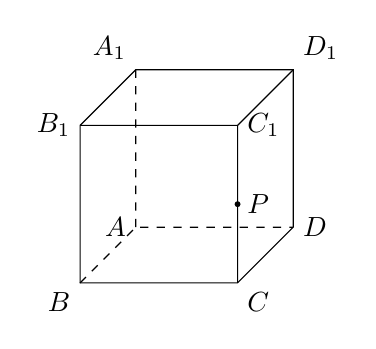
\begin{tikzpicture}
        \draw (0,0) node [below left] {$B$} coordinate (B) --++ (2,0) node [below right] {$C$} coordinate (C) --++ (45:{2/2}) node [right] {$D$} coordinate (D)
        --++ (0,2) node [above right] {$D_1$} coordinate (D1)
        --++ (-2,0) node [above left] {$A_1$} coordinate (A1) --++ (225:{2/2}) node [left] {$B_1$} coordinate (B1) -- cycle;
        \draw (B) ++ (2,2) node [right] {$C_1$} coordinate (C1) -- (C) (C1) --++ (45:{2/2}) (C1) --++ (-2,0);
        \draw [dashed] (B) --++ (45:{2/2}) node [left] {$A$} coordinate (A) --++ (2,0) (A) --++ (0,2);
        \filldraw ($(C)!0.5!(C1)$) node [right] {$P$} circle (0.03);
    \end{tikzpicture}
\end{center}
\twoch{\textcircled{1} 为真命题, \textcircled{2} 为真命题}{\textcircled{1} 为真命题, \textcircled{2} 为假命题}{\textcircled{1} 为假命题, \textcircled{2} 为真命题}{\textcircled{1} 为假命题, \textcircled{2} 为假命题}
\item 如左图, 在$\text{Rt}\triangle ABC$中, $\angle C=90^\circ$, $BC=3$, $AC=6$, $D$、$E$分别为$AC$、$AB$上的点, 且$DE\parallel BC$, $DE=2$, 将$\triangle ADE$沿$DE$折起到$\triangle A_1DE$的位置, 使$A_1C\perp CD$, 如右图.
\begin{center}
    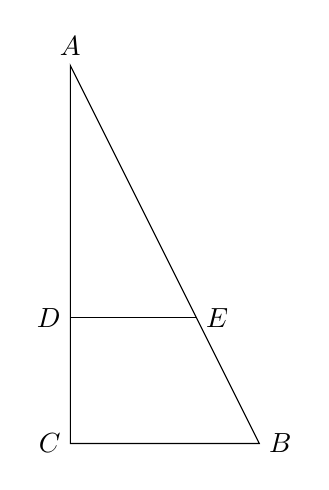
\begin{tikzpicture}[scale = 0.8]
        \draw (0,0) node [left] {$C$} coordinate (C) -- (3,0) node [right] {$B$} coordinate (B) -- (0,6) node [above] {$A$} coordinate (A) -- cycle;
        \draw ($(A)!{2/3}!(C)$) node [left] {$D$} coordinate (D) -- ($(A)!{2/3}!(B)$) node [right] {$E$} coordinate (E);
    \end{tikzpicture}
    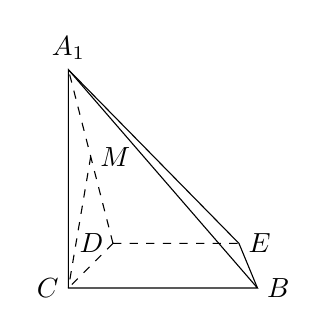
\begin{tikzpicture}[scale = 0.8]
        \draw (0,0) node [left] {$C$} coordinate (C) -- (3,0) node [right] {$B$} coordinate (B) -- (0,{2*sqrt(3)}) node [above] {$A_1$} coordinate (A1) -- cycle;
        \draw (45:1) node [left] {$D$} coordinate (D) ++ (2,0) node [right] {$E$} coordinate (E);
        \draw (B) -- (E) -- (A1);
        \draw [dashed] (D) -- (E) (D) -- (C) (D) -- (A1) ($(A1)!0.5!(D)$) node [right] {$M$} -- (C);
    \end{tikzpicture}
\end{center}
(1) 求证: $A_1C\perp$平面$BCDE$;\\
(2) 若$M$是$A_1D$的中点, 求$CM$与平面$A_1BE$所成角的大小.
\item 在$\triangle ABC$中, $a$, $b$, $c$分别是角$A$, $B$, $C$的对边, 且$8\sin^2\dfrac{B+C}2-2\cos 2A=7$.\\
(1) 求角$A$的大小;\\
(2) 若$a=\sqrt 3$, $b+c=3$, 求$b$和$c$的值.
\item 如图, $A$、$B$、$C$三地有直道相通, $AB=5$千米, $AC=3$千米, $BC=4$千米, 现甲、乙两警员同时从$A$地出发匀速前往$B$地, 经过$t$小时, 他们之间的距离为$f(t)$(单位: 千米), 甲的路线是$AB$, 速度为$5$千米/小时, 乙的路线是$ACB$, 速度为$8$千米/小时, 乙到$B$地后在原地等待, 设$t=t_1$时乙到达$C$地.
\begin{center}
    \begin{tikzpicture}[scale = 0.6]
        \draw (0,0) node [left] {$C$} -- (4,0) node [right] {$B$} -- (0,3) node [above] {$A$} -- cycle;
    \end{tikzpicture}
\end{center}
(1) 求$t_1$及$f(t_1)$的值;\\
(2) 已知警员的对讲机的有效通话距离是$3$千米, 当$t_1\le t\le 1$时, 求$f(t)$的表达式, 并判断$f(t)$在$[t_1,1]$上的最大值是否超过$3$? 说明理由.
\item 已知双曲线$\Gamma:\dfrac{x^2}2-\dfrac{y^2}4=1$的右顶点为$A$, 点$B$的坐标为$(1,\sqrt 2)$.\\
(1) 设双曲线$\Gamma$的两条渐近线的夹角为$\theta$, 求$\cos\theta$;\\
(2) 设点$D$是双曲线$\Gamma$上的动点, 若点$N$满足$\overrightarrow{BN}=\overrightarrow{ND}$, 求点$N$的轨迹方程;\\
(3) 过点$B$的动直线$l$交双曲线$\Gamma$于$PQ$两个不同的点, $M$为线段$PQ$的中点, 求直线$AM$的斜率的取值范围.
\item 记无穷数列$\{a_n\}$的前$n$项中最大值为$M_n$, 最小值为$m_n$, 令$b_n=\dfrac{M_n+m_n}{2}$.\\
(1) 若$a_n=2^n-3n$, 写出$b_1,b_2,b_3,b_4$的值;\\
(2) 设$a_n=2^n-\lambda n$, 若$b_3=-3$, 求$\lambda$的值, 及$n\ge 4$时数列$\{b_n\}$的前$n$项和$S_n$;\\
(3) 求证:``数列$\{a_n\}$是等差数列''的充要条件是``数列$\{b_n\}$是等差数列''.

\end{enumerate}
\end{document}